\documentclass[12pt,a4paper]{article}
\usepackage[utf8]{inputenc}
\usepackage[brazil]{babel}
\usepackage[left=3cm,right=3cm,top=2.5cm,bottom=2.5cm]{geometry}
\usepackage{setspace}
\usepackage{amsmath, mathrsfs, amssymb, mathtools}
\usepackage{amsthm}
\usepackage{multirow}
\usepackage{hyperref}
\usepackage{listings}
\usepackage{graphicx}
\usepackage[skip=-5pt]{caption}
\captionsetup{font={stretch=0.6,small}} 
\graphicspath{{./imagens/}}


% Custom colors
\usepackage{xcolor}

\definecolor{codegreen}{rgb}{0,0.6,0}
\definecolor{codegray}{rgb}{0.5,0.5,0.5}
\definecolor{codepurple}{rgb}{0.58,0,0.82}
\definecolor{backcolour}{rgb}{0.95,0.95,0.92}

% Python style for highlighting
\newcommand\pythonstyle{\lstset{
    language=Python,
    backgroundcolor=\color{backcolour},   
    commentstyle=\color{codegreen},
    keywordstyle=\color{magenta},
    numberstyle=\tiny\color{codegray},
    stringstyle=\color{codepurple},
    basicstyle=\ttfamily\footnotesize,
    breakatwhitespace=false,         
    breaklines=true,                 
    captionpos=b,                    
    keepspaces=true,                 
    numbers=left,                    
    numbersep=5pt,                  
    showspaces=false,                
    showstringspaces=false,
    showtabs=false,                  
    tabsize=2
}}

% Python environment
\lstnewenvironment{python}[1][]
{
\pythonstyle
\lstset{#1}
}
{}

% Python for external files
\newcommand\pythonexternal[2][]{{
\pythonstyle
\lstinputlisting[#1]{#2}}}

% Python for inline
\newcommand\pythoninline[1]{{\pythonstyle\lstinline!#1!}}

\sloppy

\title{Processamento Digital de Imagens – Trabalho 3\\Detecção de Componentes Conexos com Flood Fill}
\author{Guilherme L. Salomão, João Victor M. Freire, \\Martin Heckmann, Renan D. Pasquantonio }
\date{14 de Outubro de 2020}

\begin{document}

\maketitle

\section{Introdução}
Existem diversas formas de transformarmos uma imagem em escala de cinza em uma imagem binária, isto é, em uma imagem que só tem dois valores de intensidade. Essas são bastante úteis no processamento digital de imagens, pois é uma forma de simplificar a informação contida em tal imagem. Em particular, essa técnica é útil no processo de segmentação de objetos.

Em uma imagem binária, podemos considerar valores não nulos como objetos e, assim, é interessante descobrir o conjunto de coordenadas que o representa. Para isso utilizamos técnicas de detecção de componentes conexos.

Um componente conexo é definido como um conjunto de pixels conectados. Ou seja, definida uma vizinhança, é possível sair de um ponto $(x, y)$ do objeto e atingir todos os outros pontos dele passando apenas por vizinhos de mesma intensidade. Uma possível é a vizinhança-4, que considera como vizinhos os pixels acima, abaixo, à esquerda e à direita. A vizinhança-8 adiciona os quatro pixels da diagonal aos considerados pela 4.

\section{Motivação}

Existem métodos de extração de componentes conexos que percorrem toda a imagem categorizando todos os componentes existentes com um rótulo diferente. No entanto, esse é um algoritmo que percorre a imagem toda mais de uma vez. Em determinadas aplicações, não é necessário encontrarmos todos os componentes conexos, mas apenas encontrar um objeto inteiro.

Um exemplo de aplicação que tem essa necessidade é a ferramenta \textit{balde de tinta}, muito comum em programas de edição de imagens. Essa ferramenta, ao selecionar um pixel, altera a cor de todos os pixels adjacentes que possuem a mesma intensidade do selecionado.

O algoritmo que desempenha essa função de encontrar os pontos de um objeto, a partir de uma origem, é chamado de \textit{Flood Fill}. Sua implementação e teste será o objeto de estudo neste terceiro trabalho prático.


\section{Explicação do Método Implementado}
\subsection{Implementação com Busca em Largura}
Uma das formas de implementar o Flood Fill é através de uma busca em largura na imagem. A seguir, está uma implementação utilizando BFS e vizinhança-4.

\pythonexternal{./src/flood_fill_bfs.py}

A função \pythoninline{flood_fill()} recebe a imagem que contém o objeto e um ponto dele, chamado \pythoninline{origin}. A variável \pythoninline{obj} armazenará as coordenadas encontradas do objeto. As estruturas auxiliares \pythoninline{visited} e \pythoninline{queue} irão armazenar os pontos já visitados e uma fila de pontos que ainda devemos visitar, respectivamente.

Inicialmente colocamos a origem na fila e entramos no laço principal. Enquanto ainda houverem pontos nela, selecionamos o da frente e, caso ainda não tenha sido visitado, adicionamos ao objeto. Na primeira iteração essa operação faz sentido já que a origem é um ponto do objeto, mas para as demais devemos garantir que só pontos do objeto entrem na fila.

Para cada ponto da fila, olhamos quatro vizinhos, com coordenadas \pythoninline{up}, \pythoninline{down}, \pythoninline{left}, e \pythoninline{right}. É preciso levar em consideração pontos que podem estar na borda da imagem e que, portanto, têm apenas dois ou três vizinhos. Para isso verificamos se \pythoninline{(row, col)} tem valores \pythoninline{0}, \pythoninline{img_shape[0]-1}, ou \pythoninline{img_shape[1]-1}. Para os vizinhos válidos, devemos coloca-los na fila se ainda não foram visitados, e se tiverem a mesma intensidade da origem. Essa última verificação nos garante que todos os pontos colocados na fila cumprem os critérios para serem parte do objeto.

A seguir estão alguns testes realizados em imagens vistas em aula.

\vspace{1em}
\begin{center}
	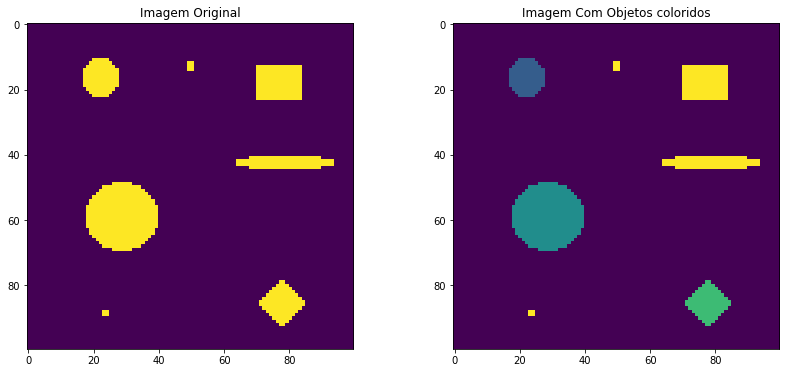
\includegraphics[width=\textwidth]{bfs_objetos1.png}
\end{center}
\vspace{1em}


\vspace{1em}
\begin{center}
	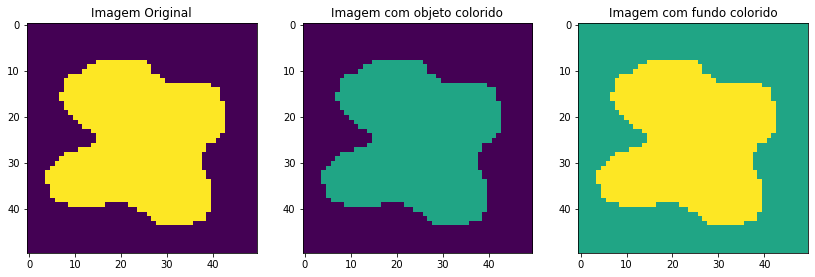
\includegraphics[width=\textwidth]{bfs_objetos2.png}
\end{center}
\vspace{1em}

\newpage

\subsection{Implementação com Busca em Profundidade}
É possível implementarmos o Flood Fill utilizando também uma busca em profundidade. Basta substituir a fila na implementação anterior por uma pilha ou utilizar a pilha da recursão. Decidimos, então, implementar uma versão recursiva do código com o objetivo de mudar a cor de um objeto, simulando o efeito \textit{balde de tinta}.

\pythonexternal{./src/flood_fill_dfs.py}

Aqui, a função recebe um ponto de origem (\pythoninline{origin}), a imagem e uma cor alternativa usada para substituir a cor original do objeto (\pythoninline{replacement}). Então, o algoritmo acessa o ponto de origem, verifica se a cor é igual a do objeto ou não é a desejada. Caso atenda essas condições, então tem sua cor trocada e a função é chamada recursivamente para seus quatro vizinhos, novamente respeitando as bordas da imagem.

\newpage

\nocite{comin2020}
\nocite{comin2021}
\nocite{wiki01}

\bibliographystyle{acm}
\bibliography{references}

\end{document}
